\subsection{Ejercicio 8}
En la presente secci�n vamos a trabajar sobre un algoritmo de scheduling de tipo Round Robin pero que no permite la migraci�n de procesos entre
n�cleos. Para tal motivo se utiliza una cola de \texttt{READY} para cada core, donde una vez que el proceso llega se moviliza s�lo por esa cola.

Cuando el proceso es bloqueado debemos tener una manera de saber a qu� CPU pertenec�a dicho proceso, y para tal fin cada core tambi�n tiene una
cola de \texttt{BLOQUED}. Entonces, cuando un proceso es desbloqueado simplemente se lo busca en alguna de las listas \texttt{BLOQUED} de los cores,
y una vez que se lo encuentra se lo agrega a la cola \texttt{READY} correspondiente al core que ten�a esa tarea bloqueada. Esto hace que cada CPU
tenga un esquema de Round Robin de un s�lo core independiente del resto.

A continuaci�n mostramos un gr�fico correspondiente al procesamiento del lote de tareas \textit{lote5.tsk} para este nuevo scheduler.

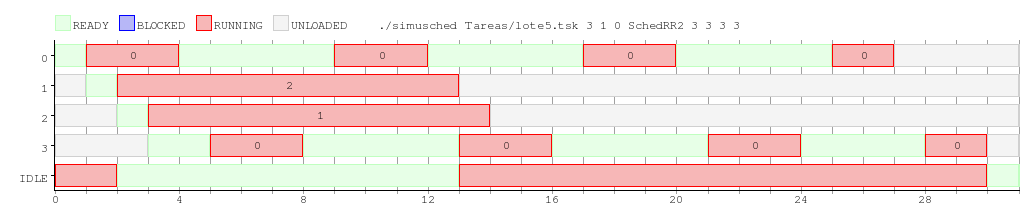
\includegraphics[width=1\textwidth]{./Graficos/ej8_1.png}
\begin{center}
 \textit{Cores = 3, Qantum = 3 cada core, CS = 1}.
\end{center}

Las dos primeras tareas llegan